\section{eo\-Init\-Adaptor$<$ EOT $>$ Class Template Reference}
\label{classeo_init_adaptor}\index{eoInitAdaptor@{eoInitAdaptor}}
eo\-Init\-Adaptor changes the place in the hierarchy from {\bf eo\-Init}{\rm (p.\,\pageref{classeo_init})} to {\bf eo\-Mon\-Op}{\rm (p.\,\pageref{classeo_mon_op})}.  


{\tt \#include $<$eo\-Init.h$>$}

Inheritance diagram for eo\-Init\-Adaptor$<$ EOT $>$::\begin{figure}[H]
\begin{center}
\leavevmode
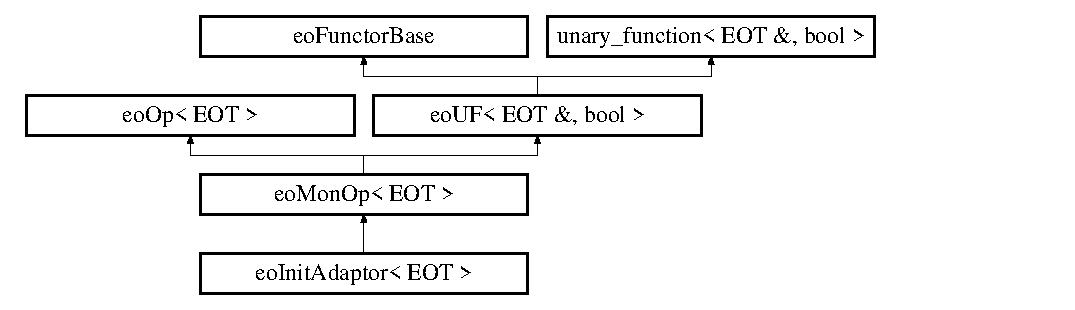
\includegraphics[height=3.71476cm]{classeo_init_adaptor}
\end{center}
\end{figure}
\subsection*{Public Member Functions}
\begin{CompactItemize}
\item 
{\bf eo\-Init\-Adaptor} ({\bf eo\-Init}$<$ {\bf EOT} $>$ \&\_\-init)\label{classeo_init_adaptor_a0}

\item 
bool {\bf operator()} ({\bf EOT} \&\_\-eot)\label{classeo_init_adaptor_a1}

\begin{CompactList}\small\item\em The pure virtual function that needs to be implemented by the subclass. \item\end{CompactList}\end{CompactItemize}
\subsection*{Private Attributes}
\begin{CompactItemize}
\item 
{\bf eo\-Init}$<$ {\bf EOT} $>$ \& {\bf init}\label{classeo_init_adaptor_r0}

\end{CompactItemize}


\subsection{Detailed Description}
\subsubsection*{template$<$class EOT$>$ class eo\-Init\-Adaptor$<$ EOT $>$}

eo\-Init\-Adaptor changes the place in the hierarchy from {\bf eo\-Init}{\rm (p.\,\pageref{classeo_init})} to {\bf eo\-Mon\-Op}{\rm (p.\,\pageref{classeo_mon_op})}. 

This is mainly a type conversion, nothing else \begin{Desc}
\item[See also:]{\bf eo\-Init}{\rm (p.\,\pageref{classeo_init})}, {\bf eo\-Mon\-Op}{\rm (p.\,\pageref{classeo_mon_op})} \end{Desc}




Definition at line 157 of file eo\-Init.h.

The documentation for this class was generated from the following file:\begin{CompactItemize}
\item 
eo\-Init.h\end{CompactItemize}
